\chapter{Szenarien im Ampelbereich}
\begin{figure}[H]  
    \centering  
    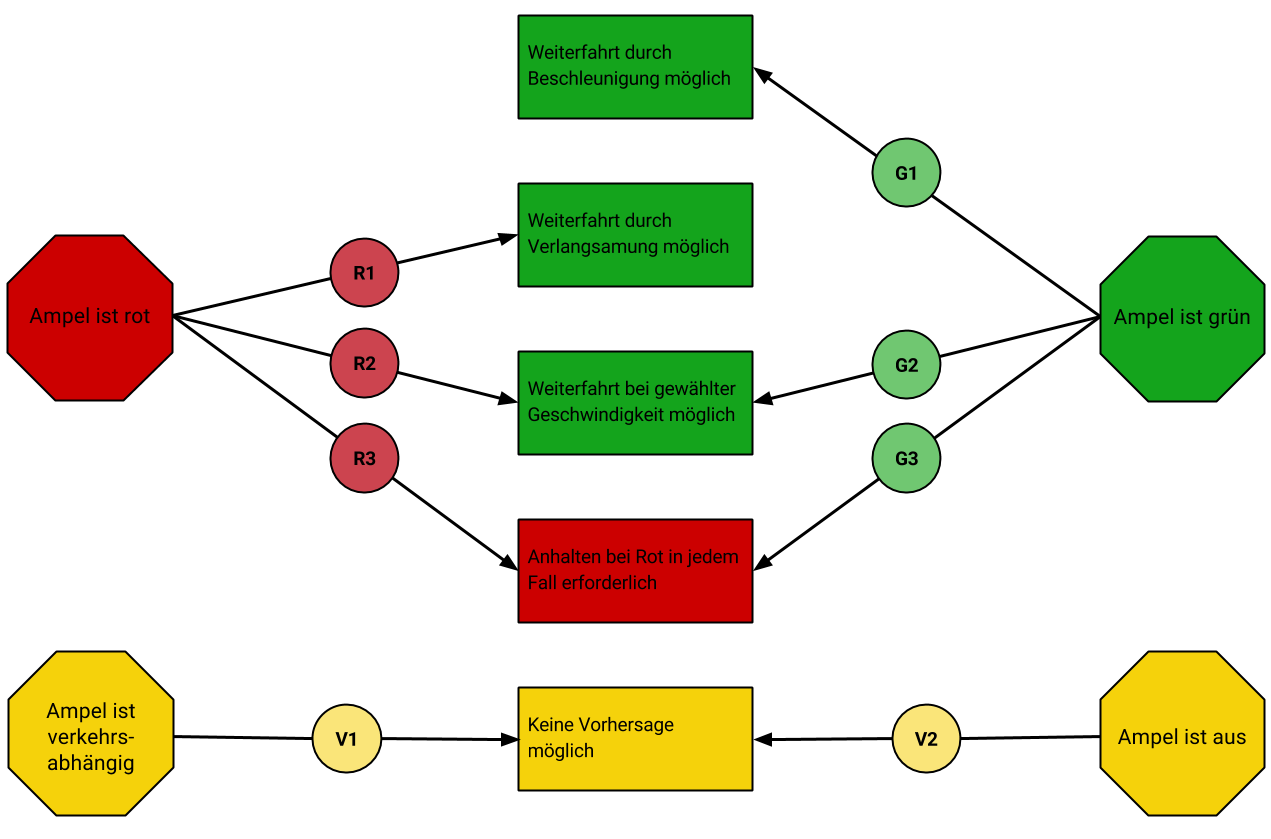
\includegraphics[width=1\textwidth]{Szenarien} 
    \label{fig:szenarien}
    \caption[Szenarien]{Szenarien im Ampelbereich}
\end{figure}
\paragraph{Anhalten ist unvermeidbar:} Die Ampelschaltung erlaubt momentan kein reibungsloses Passieren. 
\textit{Umgesetzte Anzeigevariante: \textbf{rot}}
\paragraph{Konstante Weiterfahrt möglich:} Ist die empfohlene Geschwindigkeit gleich der aktuellen, ist ein reibungsloses Passieren bei beibehaltenem Tempo möglich. Es besteht kein Handlungsbedarf. 
\textit{Umgesetzte Anzeigevariante: \textbf{grün}}
\paragraph{Reibungsloses Passieren durch Beschleunigung möglich:} Zeigt die Ampel im Moment Grün und ist die empfohlene Geschwindigkeit höher als die aktuelle, ist ein reibungsloses Passieren durch Beschleunigung zu erreichen. Bei der Anzeige der Progressionsgeschwindigkeit ist selbstverständlich die geltende Höchstgeschwindigkeitsbegrenzung zu beachten. 
\textit{Umgesetzte Anzeigevariante: \textbf{grün}}
\paragraph{Reibungsloses Passieren duch Verlangsamen möglich:} Zeigt die Ampel im Moment Rot und ist die empfohlene Geschwindigkeit niedriger als die aktuelle, ist ein reibungsloses Passieren durch Verlangsamung zu erreichen.
\textit{Umgesetzte Anzeigevariante: \textbf{grün}}
